\section{Sättigungsprozesse, beschränktes Wachstum}
\sectuntertitel{Ich kann nicht mehr...}

\subsection*{Lernziele}
\begin{itemize}
	\item Grundformel eines Sättigungsfunktion
  \item Funktionsterm bei gegebenen Randbedingungen 
\end{itemize}

Bei beschränktem Wachstum ist die Änderungsrate typischerweise
proportional zur
sog. \textbf{Sättigungsdifferenz}\index{Sättigungsdifferenz}\index{Differenz!zur Sättigung}
(auch Sättigungs\textbf{manko}\index{Sättigungsmanko}\index{Manko!der
  Sättigung} oder Sättigungsdefizit\index{Sättigungsdefizit}).
  So bezeichnet man die \textbf{Differenz} zwischen dem
  aktuellen Wert und der Sättigungsgreze.

Mit anderen Worten: Je weiter weg der aktuelle Wert vom Grenzwert ist, umso rascher ist die Zunahme (bzw. die Abnahme bei beschränktem Zerfall).

\newpage


\subsection{Beispiele von Sättigungsprozessen}
Überlegen Sie sich Beispiele von Prozessen, bei welchen eine bestimmte Schwelle nicht überschreiten bzw. unterschritten werden kann:
\begin{itemize}
	\item \Lueckentext{Laden einer Batterie (je weniger geladen, um so schneller lädt sie)}
	\item \Lueckentext{Druck ablassen aus einem Pneu (je mehr Druck, umso schneller entweicht er)}
	\item \Lueckentext{Abkühlen eines Getränks bis zur Zimmertemperatur}
	\item \Lueckentext{Aufwärmen eines Getränks auf 40 Grad Celsius}
	\item \Lueckentext{Wirkstoffniveau bei Einnahme von Medikamenten.}
	\item \Lueckentext{Populationszunahme bei beschränkten Ressourcen (Futter, Platz, ...)}
        \item \Lueckentext{Lernkurve}
        \item \Lueckentext{\dotfill}
\end{itemize}
\newpage


\subsection{Begrenzter Zerfall}\index{Begrenzter Zerfall}\index{Zerfall!begrenzter}

\subsubsection{Einstiegsbeispiel Tee}\index{Tee!Abkühlungsprozess}\index{Abkühlungsprozess}

Tee wird von 75 Grad Celsius auf Zimmertemperatur (20 Grad)
abgekühlt. Nach drei Minuten messen wir 61 Grad.


a) Skizzieren Sie die «Zerfallskurve», welche die Temperatur des Tees
angibt.

b) Geben Sie die Funktionsgleichung $f(t)$ an, welche den Prozess
beschreibt.

c) Wie warm ist der Tee nach 5 Minuten?  

d) Wann ist die Temperatur auf angenehme 37 Grad gesunken?

\noTRAINER{\bbwCenterGraphic{17cm}{allg/funktionen/img/saettigung/Tee.png}}

\TNTeop{a) Idee mit gleicher Formel klappt nicht, denn der
  Standard-Exponentielle Zerfall geht nach Null!

  Skizze mit 75 Grad, 20 Grad (Sättigung) und 61 Grad.

Idee: verschiebe die Skala um 20 Einheiten nach unten. Nun
funktioniert es: $g(t) = 55\cdot{}\left(\frac{41}{55}\right)^{\frac{t}{3}}$

Verschiebe wieder zurück: ACHTUNG: Das $b$ ist nun jedoch die
Sättigungs\textbf{differenz} zum Zeitpunkt $t_0=0$ und \textbf{nicht} mehr der Startwert! 

b)
$$f(t) = 20 + g(t) = 20 + 55\cdot{}\left(\frac{41}{55}\right)^{\frac{t}{3}}$$

c) $f(5) = 20 + 55\cdot{} \left(\frac{41}{55}\right)^{\frac{5}{3}}
\approx  53.7\degre$

d) Berechnung: Wann sind 37 Grad erreicht? Einsetzen
in die Funktionsgleichung:

$$37\degre = y=f(t) = 20 + 55\cdot{}\left(\frac{41}{55}\right)^{\frac{t}{3}}$$

Solver (num-solv):
$$37\degre 20 + 55\cdot{}\left(\frac{41}{55}\right)^{\frac{x}{3}}$$

$$\Longrightarrow t \approx 11.99 \text{ min}$$


}%% END TNT

\newpage

\subsubsection{Allgemeine Form des beschränkten Zerfalls}
\begin{center}
\raisebox{-1cm}{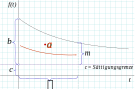
\includegraphics[width=13cm]{allg/funktionen/img/saettigung/saettigungskurveDown.png}}
\end{center}

Die Grundform eines begrenzten Zerfalls ist ein normaler
exponentieller Zerfall ($y=a^{t}$, $0<a<1$), der in $y$-Richtung um
eine Sättigungsgrenze $c$
(\textit{capacity}\index{capacity $c$}\index{Kapazität (capacity)})verschoben ist:

\begin{gesetz}{beschränkter Zerfall}{}\index{beschränkter Zerfall}\index{Zerfall!beschränkter}
  Grundform des beschränkten Zerfalls:
$$f(t) = c + b\cdot{}a^{\frac{t}{\tau}}$$
\end{gesetz}

Dabei ist:
\begin{itemize}
  \item $c+b = f(0) = y$-Achsenabschnitt = Startwert
	\item $c$: Die Sättigungsgrenze\index{Sättigungsgrenze} (Sättigungswert). Dies ist die Annäherungskonstante oder der \textbf{Asymtote}nwert\index{Asymptote}: Tiefer kann die Funktion nicht fallen.

	\item $m$:
    Sättigungs\textbf{differenz}\index{Sättigungsdifferenz}\index{Differenz!zur Sättigung}. Wie viel fehlt, bis zur
    Sättigungsgrenze: $m = f(t) - c$. Die Sättigungs\textbf{differenz} nimmt exponentiell ab.
	\item $b$: Die \textbf{Abweichung} zu $c$ zum Zeitpunkt $t=0$. Der
    Anfangswert ist somit $f(0) = c + b$; mit anderen Worten: $b$ ist das
    \textbf{Sättigungsdifferenz} zum Zeitpunkt $t_0 = 0$.

    \item $a=\frac{m}{b}=\frac{f(\tau)-c}{f(0)-c}$: Der Faktor der Veränderung der
      Sättigung\textbf{differenz}.
\end{itemize}
\newpage


\subsection*{Aufgaben}

\GESO{\olatLinkArbeitsblatt{Exponentialfunktionen}{https://olat.bms-w.ch/auth/RepositoryEntry/6029794/CourseNode/106029175831971}{Kap. 3.1:
    Sättigung: Begrenzter Zerfall}}
\TALS{\olatLinkArbeitsblatt{Exponentialfunktionen}{https://olat.bms-w.ch/auth/RepositoryEntry/6029786/CourseNode/106029175777725}{Kap. 3.:
    Sättigung: Begrenzter Zerfall}}


\GESOAadBMTA{359}{35. (Kuchen) und 36. (Ovomaltine)}
\olatLinkGESOKompendium{3.4.2}{33}{48. (Achtung: Das
  Kompendium verwendet andere Buchstaben: Das dortige $a$ ist unser $b$.)}
\newpage


\subsection{Sättigung (begrenztes Wachstum)}\index{Sättigung}\index{begrenztes Wachstum}\index{Wachstum!begrenztes}
\subsubsection{Einstiegsbeispiel 1: Eistee wärmen}
Das Aufwärmen von Eistee von $5\degre$ Kühlschranktemperatur auf $20\degre$ Zimmertemperatur ist ein klassisches «Begrenztes Wachstum» (mit gespiegelter Exponentialfunktion).

\TNT{5.2}{Skizze}

\subsubsection{Einstiegsbeispiel 2: Batterie laden}
\begin{center}
\raisebox{-1cm}{
\includegraphics[width=8cm]{allg/funktionen/img/saettigung/batterien.png}}
\end{center}

Eine 9V-Batterie ist etwas mehr als zur Hälfte entladen und enthält nun eine
Restspannung von 4V.

Wenn wir 9V an die Batterie anlegen, so wird die Batterie geladen.

Die Batterie lädt sich umso rascher, je \textit{leerer} sie ist.

Die Batterie lädt sich umso langsamer, je \textit{voller} sie ist.


\newpage

\subsubsection{Allgemeine Form von Sättigungsprozessen}

\begin{center}
\raisebox{-1cm}{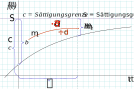
\includegraphics[width=13cm]{allg/funktionen/img/saettigung/saettigungskurve.png}}
\end{center}

Die Grundform des begrenzten Wachstums ist ein exponentieller Zerfall\totalref{zerfallsfunktion},
der an der $x$-Achse gespiegelt und in $y$-Richtung
verschoben ist:

\begin{gesetz}{Sättigung}{}
  Grundform beschränktes Wachstum:
$$f(t) =c - b\cdot{} a^{\frac{t}{\tau}}$$
\end{gesetz}

Die Variable haben die folgenden Bedeutungen:

\begin{itemize}
	\item $c$: Sättigungsgrenze. Dies ist die Annäherungskonstante oder der Asymtotenwert. Höher kann die Funktion nicht steigen.

	\item $m$ ist die
    Sättigungsdifferenz\index{Sättigungsdifferenz}\index{Differenz!zur Sättigung}. Wie viel fehlt, bis zur
    Sättigungsgrenze: $m = c - f(t)$. Auch hier nimmt die Sättigungs\textbf{differenz} exponentiell ab.
	\item $b$: Die Abweichung des Funktionsgraphen zu $S$ zum Zeitpunkt $t=0$. Der
    Anfangswert ist somit $f(0) = c - b$.
\item $a=\frac{m}{b}=\frac{c-f(\tau)}{c-f(0)}$ Faktor der Veränderung
  der Sättigungs\textbf{differenz}.
\end{itemize}


\newpage

\subsection{Referenzaufgaben}

\subsubsection{Berechnung am Batterie-Beispiel}\index{Batterie}
Eine Batterie weist zum Zeitpunkt $t_0$ vier Volt auf. Nach sechs Stunden am Ladegerät zeigt die Messung sieben Volt. Wir wissen, dass die Sättigungsgrenze (Ladespannung) bei neun Volt liegt.

Zeichnen Sie die gegebenen Größen in ein Koordinatensystem ein und markieren Sie bei neun Volt eine horizontale Beschränkungslinie (\zB 1V = 1 Häus'chen in $y$-Richtung; 1h = 1 Häus'chen in $x$-Richtung).

\noTRAINER{\bbwCenterGraphic{15cm}{allg/funktionen/img/saettigung/batterieFctLeer.png}}
\TRAINER{\bbwCenterGraphic{15cm}{allg/funktionen/img/saettigung/batterieFct.png}}

\textbf{Frage 1}: Wie lautet die Formel $f(t) = ...$ der Sättigungskurve?

\noTRAINER{$c = ..........................$}
\TRAINER{$c = \text{ Sättigungsgrenze } = 9 [\text{V}]$}

\noTRAINER{$b = ..........................$}
\TRAINER{$b = m_0 = c-f(0) = 9 - 4 = 5$}

\noTRAINER{$\tau = .........................$}
\TRAINER{$\tau = 6$ ($e_x$ = eine Stunde)}

\noTRAINER{$m =  ..........................$}
\TRAINER{$m = m_\tau = c-f(\tau) = 9 - 7 = 2$}

\noTRAINER{$a = .........................$}
\TRAINER{$a=\frac{m}{b} = \frac{m_\tau}{m_0} = \frac{2}{5} = 0.4$}


\noTRAINER{$f(t) = c - b\cdot{}a^{\frac{t}{\tau}} = ..... - .....\cdot{}(.....)^{\frac{t}{.....}}$}
\TRAINER{$f(t) = c - b\cdot{}a^{\frac{t}{\tau}} = 9 - 5\cdot{}(\frac{2}{5})^{\frac{t}{6}}$}

\TRAINER{Die Kontrollen für $t=0$ und $t=6$ sind mit dem Stehenlassen von $a$ als Bruch nun sehr einfach.}
\newpage

\textbf{Frage 2}: Wann wird die Batterie zu 99\% geladen sein?

\TNTeop{99\% von 9V = 8.91 V

  Somit ist $t$ gesucht mit $f(t) = 9 - 5\cdot{}\left(\frac25\right)^{\frac{t}{6}} = 8.91$

  (beidseitig -9 und Vorzeichen drehen und dann durch 5 teilen, so folgt...)

  $$(0.4)^{\frac{t}{6}} = (9-8.91) : 5 = 0.09 : 5 = 0.018$$

  Definition Logarithmus:

  $$\frac{t}6 = \log_{0.4}(0.018) \approx 26.3 $$

  Nach ca. 26 - 27 Stunden ist die Batterie zu 99\% geladen.
}
\newpage

\subsubsection{Bemerkungen}
\begin{bemerkung}{}{}
  Für die Sättigungsdifferenzen $m_0$ und $m_\tau$ gilt:
  $$m_0 = m(0) = c- f(0) = c- (c-b\cdot{}a^0) = c-(c-b) = b$$

  und

  $$\frac{m_\tau}{m_0} = \frac{c-f(\tau)}{b} =
  \frac{c-(c-b\cdot{}a^\frac{\tau}{\tau})}{b}  = \frac{+b\cdot{}a}{b} = a$$
\end{bemerkung}

\TRAINER{ Bemerkung (Trainer/mündlich):
  
Das $a$ kann aus zwei \textbf{beliebigen} Sättigungsdifferenz-Werten berechnet werden (die um die
Zeitdifferenz $\tau$ auseinander liegen):
$$\frac{m_2}{m_1} = \frac{b\cdot{}a^{\frac{t_2}{\tau}}}{b\cdot{}
  a^{\frac{t_1}{\tau}}} = a^{\frac{t_2}{\tau}} : a^{\frac{t_1}{\tau}} =
a^{\frac{t_2-t_1}{\tau}} = a^{\frac{\tau}{\tau}} = a$$%% 
}%% END Trainer


\begin{bemerkung}{}{}
Meistens ist $m_0$ zum Zeitpunkt $t=0$ bekannt und somit ist $b=m_0$. Es reicht, die Messung zum Zeitpunkt $t_0$ und zu einem weiteren Zeitpunkt durchzuführen. Wenn zusätzlich die Sättigungsgrenze $c$ bekannt ist, kann die Funktion $f$ komplett bestimmt werden.
\end{bemerkung} 

\newpage
\subsubsection{Referenzaufgabe Sättigung: Pneu (optional)}\index{Reifen}\index{Pneu}

Ein Reifen (Pneu) ist anfänglich ganz leer und enthält «nur» 1 atm, nämlich den
Druck der Umgebung. (1 atm = atmosphärischer Druck = technische Atmosphäre) 

Der Reifen wird aufgepumpt mit einer Druckpumpe, die maximal 2 atm
leisten
kann. Mit 2 atm ist hier gemeint: 2 at mehr als der
Umgebungsdruck. Somit könnte der Pneu bis auf maximal 3 atm aufgepumpt
werden (= Sättigungsgrenze).

Um den Reifen optimal zu füllen, wird er auf 2 atm aufgepumpt (1 atm
über dem Umgebungsluftdruck).

Die Pumpe schafft in den ersten 10 Sekunden den Druck von 1 atm auf 1.2
atm (= 0.2 atm über Normaldruck) aufzupumpen.

Nach wie vielen Sekunden muss gestoppt werden, damit der Reifen
optimal gepumpt ist?

\TNTeop{Die Sättigungsdifferenz schwindet von $m_1=3-1=2$ bis $m_2=3-1.2=1.8$
innerhalb der ersten $10s = \tau$. Die Sättigungsgrenze liegt bei
$S=3$. Unsere (Exponential)basis $a$ ist somit $1.8 / 2$, was uns
liefert:
$$f(t) = 3 - 2\cdot{}\left(\frac{1.8}{2}\right)^\frac{t}{10}$$
Somit ist das Optimum bei $2 = 3-
2\cdot{}\left(\frac{1.8}{2}\right)^\frac{t}{10}$ erreicht, also bei
etwa 65.8 Sekunden.
}
\newpage

\subsection*{Aufgaben}

\GESO{\olatLinkArbeitsblatt{Exponentialfunktionen}{https://olat.bms-w.ch/auth/RepositoryEntry/6029794/CourseNode/106029175831971}{Kap. 3.2:
    Begrenztes Wachstum}}%% END GESO
\TALS{\olatLinkArbeitsblatt{Exponentialfunktionen}{https://olat.bms-w.ch/auth/RepositoryEntry/6029786/CourseNode/106029175777725}{Kap. 3.2:
    Begrenztes Wachstum}}%% END TALS

%%\GESOAadBMTA{358}{34. (Eistee)} entfernt, da Aufgabe «Cola» ist identisch
\olatLinkGESOKompendium{3.4.2}{32ff}{49. - 51. (Bem.: Dasf
  Kompendium gibt die Funktionsterme bereits an und verwendet als
  Basis i.\,d.\,R. die Eulersche Konstante $e\approx{} 2.71828$)}

\newpage

\subsection{Zusammenfassung der Prozesse}
\vspace{8mm}
\begin{center}\textbf{Wachstum und Zerfall}\end{center}


\noTRAINER{\begin{tabular}{cc}
    \bbwGraph{-3}{4}{-1}{4}{} &
    \bbwGraph{-3}{4}{-1}{4}{} \\
\end{tabular}}%% end noTRAINER
\TRAINER{\bbwCenterGraphic{18cm}{allg/funktionen/img/zusammenfassung_exp/wachstum_zerfall.png}

  bzw.
  $$f(t) = G_0 \cdot{} \e^{qt}; q=  \frac{\ln(a)}\tau  \,\,\,\,\,\,\,\,\, f(t) = G_0 \cdot{} \e^{-qt}; q  = \frac{-\ln(a)}\tau$$
}%% END TNT

\vspace{8mm}
\begin{center}\textbf{Sättigung}\end{center}

\noTRAINER{\begin{tabular}{cc}
    \bbwGraph{-3}{4}{-1}{6}{} &
    \bbwGraph{-3}{4}{-1}{6}{} \\
\end{tabular}}%% end noTRAINER
\TRAINER{\bbwCenterGraphic{18cm}{allg/funktionen/img/zusammenfassung_exp/saettigung.png}

    bzw.
     $$f(t) = S + (G_0-S) \cdot{} \e^{q\cdot{}t}; q=    \frac{\ln(a)}\tau     \,\,\,\,\,\,\,\,\, f(t) = S + (S - G_0) \cdot{} \e^{-q\cdot{}t}; q  = \frac{-\ln(a)}\tau$$

Hier ist Platz für das Video/die Videos zur den getanzten
Funktionen (S. OLAT/Wiki).
}%% Trainer
\newpage

\begin{rezept}{Exponentielle Prozesse}{}
  \begin{itemize}
  \item Asymptote $c$ suchen (meist 0)
  \item $f(0)$, $\tau$ und $f(\tau)$ aus dem Text ablesen
  \item $b := f(0)- c$ (Bei gesättigtem Wachstum ist $b<0$)
  \item $m := f(\tau) - c$
  \item $a := \frac{m}{b}$ (Test: Nur bei unbeschränktem Wachstum ist
    $a>1$. Sonst gilt immer $0 < a < 1$.)
  \item $f(t) = c+b\cdot{}a^{\frac{t}{\tau}} = c + b\cdot{} e^{\frac{t\cdot{}\ln(a)}{\tau}}$
    \end{itemize} 
\end{rezept}

\newpage

\TALS{
  \subsection*{Aufgaben}
  \olatLinkTALSStrukturaufgabenSPF{Basiskenntnisse Funktionen Teil
    1}{5}{4., 5., 8. und 9.}
  \olatLinkTALSStrukturaufgabenSPF{Basiskenntnisse Funktionen Teil
    2}{14}{45., 47. und 49.}
}%% END TALS
